\documentclass{beamer}

% Theme
\usetheme{Madrid}
\usecolortheme{default}
\usemintedstyle{friendly}

% Packages
\usepackage{amsmath,amssymb,amsfonts}
\usepackage{graphicx}
\usepackage{xcolor}
\usepackage{tikz}
\usepackage{tkz-euclide}
\usepackage{array}
\usepackage{multirow}
\usepackage{longtable}
\usepackage{lscape}
\usepackage{minted}
\usepackage{graphicx}                    
\usepackage{fancyvrb}                    
\usepackage{xcolor}

% Custom macros
\newcommand{\myvec}[1]{\begin{pmatrix}#1\end{pmatrix}}
\newcommand{\brak}[1]{\left( #1 \right)}

% Redefine \vec to bold letters only (no arrow)
\renewcommand{\vec}[1]{\mathbf{#1}}

\title{1.9.8}
\author{EE25BTECH11019 -- Darji Vivek M.}
\date{}

\begin{document}

% Title slide
\begin{frame}
  \titlepage
\end{frame}

% Question slide
\begin{frame}{Question}
The distance between the points 
\(\brak{0,0}\) and \(\brak{a-b,\,a+b}\) is 
\underline{\hspace{2cm}} 
\hfill $\brak{10,2021}$
\end{frame}

% Variables table
\begin{frame}{Variables Used}
\begin{table}[h!]    
  \centering
  \begin{tabular}{|c|c|}
    \hline
    Symbol & Meaning \\ \hline
    $\vec{A}$ & Point $(0,0)$ \\ \hline
    $\vec{B}$ & Point $(a-b,\,a+b)$ \\ \hline
    $a,b$ & Parameters \\ \hline
    $d$ & Distance between points \\ \hline
  \end{tabular}
\end{table}
\end{frame}

% Distance formula
\begin{frame}{Distance Formula}
\begin{align}
\vec{A} &= \myvec{0\\0}, \quad
\vec{B} = \myvec{a-b\\a+b} \\[2mm]
d &= \norm{\vec{A}-\vec{B}}
\end{align}
\end{frame}

% Substitution
\begin{frame}{Substitution}
\begin{align}
d &= \norm{\myvec{0\\0}-\myvec{a-b\\a+b}} \\
  &= \norm{\myvec{-(a-b)\\-(a+b)}} \\
  &= \sqrt{(a-b)^2 + (a+b)^2}
\end{align}
\end{frame}

% Simplification
\begin{frame}{Simplification}
\begin{align}
d &= \sqrt{a^2 - 2ab + b^2 + a^2 + 2ab + b^2} \\
  &= \sqrt{2a^2 + 2b^2} \\
  &= \sqrt{2}\sqrt{a^2+b^2}
\end{align}
\end{frame}

% Final Answer
\begin{frame}{Final Answer}
\[
\boxed{d = \sqrt{2}\sqrt{a^2+b^2}}
\]
\end{frame}

\begin{frame}[fragile]{C Function: Compute Distance Between Points}
\begin{minted}{c}
#include <math.h>

// Function to compute distance between (0,0) and (a-b, a+b)
double find_distance(double a, double b) {
    double x = a - b;
    double y = a + b;
    return sqrt(x*x + y*y);
}
\end{minted}
\end{frame}

%------------------------------------------------
\begin{frame}[fragile]{Compile C Code as Shared Library}
\begin{minted}{bash}
gcc -shared -o 2.so -fPIC 2.c -lm
\end{minted}
\end{frame}

%------------------------------------------------
\begin{frame}[fragile]{Python: Load C Library}
\begin{minted}{python}
import ctypes
import numpy as np
import matplotlib.pyplot as plt

# Load the shared library
lib = ctypes.CDLL('./2.so')

# Define function signature (double, double) -> double
lib.find_distance.argtypes = [ctypes.c_double, ctypes.c_double]
lib.find_distance.restype = ctypes.c_double
\end{minted}
\end{frame}

%------------------------------------------------
\begin{frame}[fragile]{Python: Call C Function}
\begin{minted}{python}
# Example input values
a, b = 5, 2   # can change these

# Call C function
dist = lib.find_distance(a, b)
print(f"Distance between (0,0) and ({a-b},{a+b}) = {dist:.2f}")
\end{minted}
\end{frame}

%------------------------------------------------
\begin{frame}[fragile]{Python: Define Points for Plot}
\begin{minted}{python}
# Define points
A = np.array([0, 0])               # Origin
B = np.array([a - b, a + b])       # Point (a-b, a+b)
\end{minted}
\end{frame}

%------------------------------------------------
\begin{frame}[fragile]{Python: Plot Line and Points}
\begin{minted}{python}
# Plot line AB
plt.plot([A[0], B[0]], [A[1], B[1]], 'k-', label='$AB$')

# Plot points
plt.scatter([A[0], B[0]], [A[1], B[1]], c=['red', 'blue'])
labels = ['A(0,0)', f'B({a-b},{a+b})']
coords = [A, B]

# Annotate points
for label, coord in zip(labels, coords):
    plt.annotate(
        label,
        (coord[0], coord[1]),
        textcoords="offset points",
        xytext=(10, -10),
        ha='center'
    )
\end{minted}
\end{frame}

%------------------------------------------------
\begin{frame}[fragile]{Python: Decorations and Save Figure}
\begin{minted}{python}
# Decorations
plt.legend()
plt.grid(True)
plt.axis('equal')
plt.title(f"Distance = {dist:.2f}")

# Save figure
plt.savefig("2.png", dpi=150)
plt.show()
\end{minted}
\end{frame}
\begin{frame}{plot}
\begin{figure}[H]
\centering
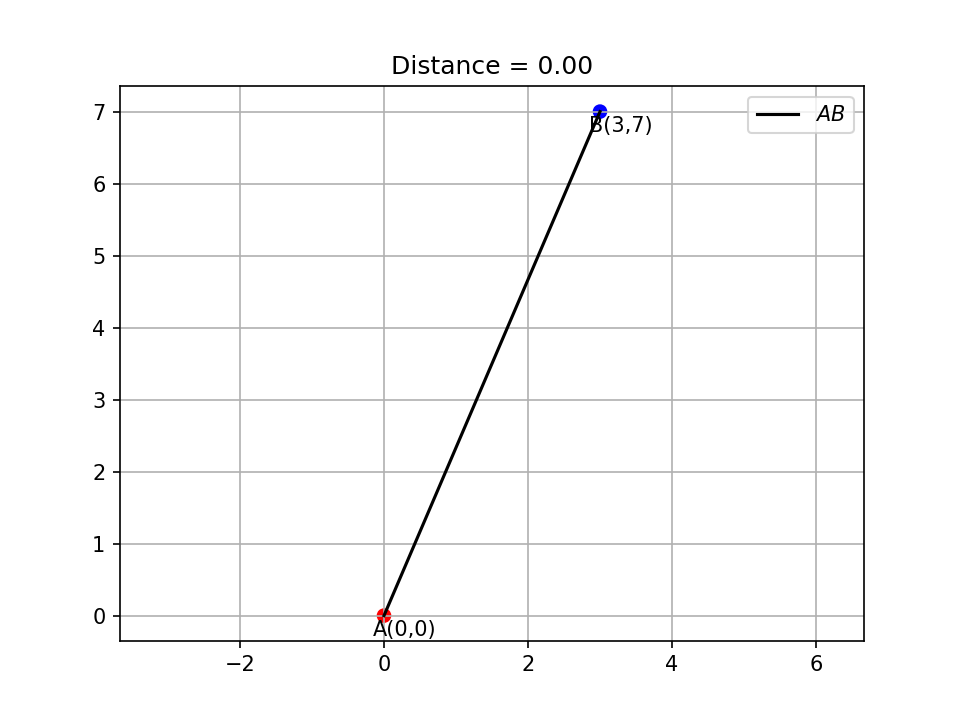
\includegraphics[width=0.75\columnwidth]{figs/2.png}
\caption{\centering plot}
\label{fig:placeholder_125}
\end{figure}
\end{frame}
\end{document}
